\documentclass[a4paper,12pt]{article}
\usepackage[T2A]{fontenc}
\usepackage[utf8]{inputenc}
\usepackage[english,russian]{babel}
\usepackage{listings}

\usepackage[table]{xcolor}

\usepackage{amsmath}
\usepackage{MnSymbol}
\usepackage{wasysym}
\usepackage{indentfirst}
\usepackage[unicode, pdftex]{hyperref}

\usepackage{pgfplots}
\pgfplotsset{compat=1.9}

\usepackage{geometry}
\geometry{left=2cm}
\geometry{right=1.5cm}
\geometry{top=1cm}
\geometry{bottom=2cm}

\usepackage{graphicx}
\graphicspath{{img/}}
\DeclareGraphicsExtensions{.pdf,.png,.jpg}

\usepackage{float}

\newcommand{\anonsection}[1]{\section*{#1}\addcontentsline{toc}{section}{#1}}

% переименовываем  список литературы в "список используемой литературы"
\addto\captionsrussian{\def\refname{Список используемой литературы}}

\lstset{
    language=C++,
    numbers=left,
    frame=single,
    texcl=true,
    basicstyle=\ttfamily
}

\begin{document}

\begin{titlepage}

    \begin{center}
        \large
        Государственное образовательное учреждение высшего профессионального образования\\
        “Московский государственный технический университет имени Н.Э.Баумана”
        \vspace{3cm}

        \textsc{Дисциплина: Анализ алгоритмов}
        \vspace{0.5cm}

        \textsc{Лабораторная работа №7}
        \vspace{3cm}

        {\LARGE АЛГОРИТМЫ СРАВНЕНИЯ С ОБРАЗЦОМ}
        \vspace{3cm}

        Студент группы ИУ7-53,\\
        Степанов Александр Олегович
        \vfill
    \end{center}

    \begin{flushright}
        \begin{tabular}{l}
            Преподаватели:\\
            Строганов Юрий Владимирович\\
            Волкова Лилия Леонидовна
        \end{tabular}
    \end{flushright}

    \begin{center}

        2019 г.

    \end{center}

\end{titlepage}

\tableofcontents

\newpage
\anonsection{Введение}

Те, кому приходиться часто работать с текстовыми редакторами,
часто пользуются функцией нахождения слов в тексте,
которая существенно облегчает редактирование документов и
поиск нужной информации. Все современные текстовые редакторы
поддерживают функционал поиска и замены
текстовых фрагментов \cite{office}.

Функции поиска входят во многие языки
программирования высокого уровня – чтобы найти строчку
в небольшом тексте используется встроенная функция \cite{cpp}.

Цель данной работы изучить и разработать алгоритм поиска
подстроки в строке.

Задачи данной работы:

\begin{itemize}
    \item изучить основные алгоритмы, решающих задачу поиска;
    \item реализовать данные алгоритмы.
\end{itemize}

\newpage
\section{Аналитическая часть}

Изучим алгоритмы поиска подстроки в строке.

\subsection{Описание задачи}

Поиск строки формально определяется следующим образом. Пусть задан массив$S$ элементов и массив $X$ элементов. Поиск строки обнаруживает первое вхождение $X$ в $S$, результатом будем считать индекс $i$, указы- вающий на первое с начала строки (с начала массива $S$) совпадение со словом.

\subsection{Пути решения}

\subsubsection{Алгоритм Кнута-Морриса-Пратта}

Алгоритм был разработан Кнутом и Праттом и независимо от них
Моррисом в 1977 г.

После частичного совпадения начальной части подстроки $X$ с
соответствующими символами строки $S$ мы фактически знаем
пройденную часть строки и может «вычислить» некоторые сведения
(на основе самого подстроки $X$), с помощью которых потом быстро
продвинемся по тексту.

Идея КМП-поиска -- при каждом несовпадении двух символов текста и
образа образ сдвигается на самое длинное совпадение начала с концом
префикса (не учитывая тривиальное совпадение самого с собой)

\paragraph{Пример}

Создается массив сдвигов (таблица \ref{table:example1}).

\begin{table}[H]
    \centering
    \caption{Массив сдвигов}
    \label{table:example1}
    \begin{tabular}{|c|c|c|l|l|l|}
    \hline
    0 & 1 & 2 & 3 & 4 & 5 \\ \hline
    a & b & c & a & b & d \\ \hline
    0 & 0 & 0 & 1 & 2 & 0 \\ \hline
    \end{tabular}
\end{table}

В таблице \ref{table:kmp} представлена работа алгоритма.

\begin{table}[H]
    \centering
    \caption{Алгоритм КМП}
    \label{table:kmp}
    \begin{tabular}{|l|l|l|l|l|l|l|l|l|l|l|l|l|l|l|l|}
    \hline
    cтрока & a & b & c & a & b & e  & a & b & c & a & b & c & a & b & d\\
    \hline
    подстрока & a & b & c & a & b & \cellcolor[HTML]{FE0000}d & & & & & & & & & \\
    \hline
    подстрока & & & & a & b & \cellcolor[HTML]{FE0000}c & a & b & d & & & & & & \\
    \hline
    подстрока & & & & & & \cellcolor[HTML]{FE0000}a & b & c & a & b & d & & & & \\
    \hline
    подстрока & & & & & & & a & b & c & a & b & \cellcolor[HTML]{FE0000}d & & & \\
    \hline
    подстрока & & & & & & & & & & \cellcolor[HTML]{34FF34}a & \cellcolor[HTML]{34FF34}b & \cellcolor[HTML]{34FF34}c & \cellcolor[HTML]{34FF34}a & \cellcolor[HTML]{34FF34}b & \cellcolor[HTML]{34FF34}d \\
    \hline
    \end{tabular}
\end{table}

\subsubsection{Алгоритм Бойера-Мура}

Алгоритм поиска строки Бойера -- Мура считается наиболее быстрым
среди алгоритмов общего назначения, предназначенных для поиска
подстроки в строке. Был разработан Бойером и Муром в 1977 году.
Преимущество этого алгоритма в том, что ценой некоторого количества
предварительных вычислений над шаблоном (но не над строкой, в которой
ведётся поиск) шаблон сравнивается с исходным текстом не во всех
позициях -- часть проверок пропускаются как заведомо не дающие
результата.

Основная идея алгоритма -- начать поиск не с начала, а с конца
подстроки. Наткнувшись на несовпадение, мы просто смещаем подстроку
до самого правого вхождения данного символа, не учитывая последний.

\paragraph{Пример}

Создается массив прыжков (таблица \ref{table:example2}).

\begin{table}[H]
    \centering
    \caption{Массив прыжков}
    \label{table:example2}
    \begin{tabular}{|c|c|c|l|l|l|}
    \hline
    0 & 1 & 2 & 3 & 4 & 5 \\ \hline
    a & b & c & a & b & d \\ \hline
    0 & 0 & 0 & 1 & 2 & 0 \\ \hline
    \end{tabular}
\end{table}

В таблице \ref{table:bm} представлена работа алгоритма.

\begin{table}[H]
    \centering
    \caption{Алгоритм БМ}
    \label{table:bm}
    \begin{tabular}{|l|l|l|l|l|l|l|l|l|l|l|l|l|l|l|l|}
    \hline
    cтрока & a & b & c & a & b & e & a & b & c & a & b & c & a & b & d \\
    \hline
    подстрока & a & b & c & a & b & \cellcolor[HTML]{FE0000}d & & & & & & & & & \\
    \hline
    подстрока & & & & & & & a & b & c & a & b & \cellcolor[HTML]{FE0000}d & & & \\
    \hline
    подстрока & & & & & & & & & & \cellcolor[HTML]{34FF34}a & \cellcolor[HTML]{34FF34}b & \cellcolor[HTML]{34FF34}c & \cellcolor[HTML]{34FF34}a & \cellcolor[HTML]{34FF34}b & \cellcolor[HTML]{34FF34}d \\
    \hline
    \end{tabular}
\end{table}

\subsection{Выводы}

Изучены алгоритмы поиска подстроки в строке, необходимо реализовать их.

\newpage
\section{Конструкторская часть}

Рассмотрим алгоритмы поиска подстроки в строке.

\subsection{Функциональная модель}

На рисунке \ref{img:idef0} представлена функциональная модель IDEF0
первого уровня.

\begin{figure}[H]
    \centering
    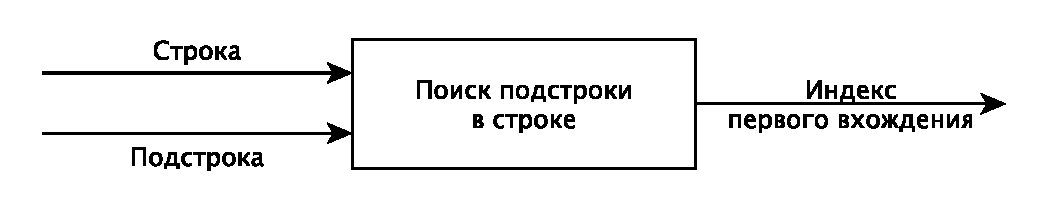
\includegraphics[scale=0.9]{idef0}
    \caption{IDEF0 первого уговня}
    \label{img:idef0}
\end{figure}

\subsection{Схемы алгоритмов}

На рисунках \ref{img:kmp} и \ref{img:bm} представлены схемы алгоритмов.
На рисунке \ref{img:fail} представлена схема создания массива сдвигов
для алгоримта Кнута-Морриса-Пратта.

\begin{figure}[H]
    \centering
    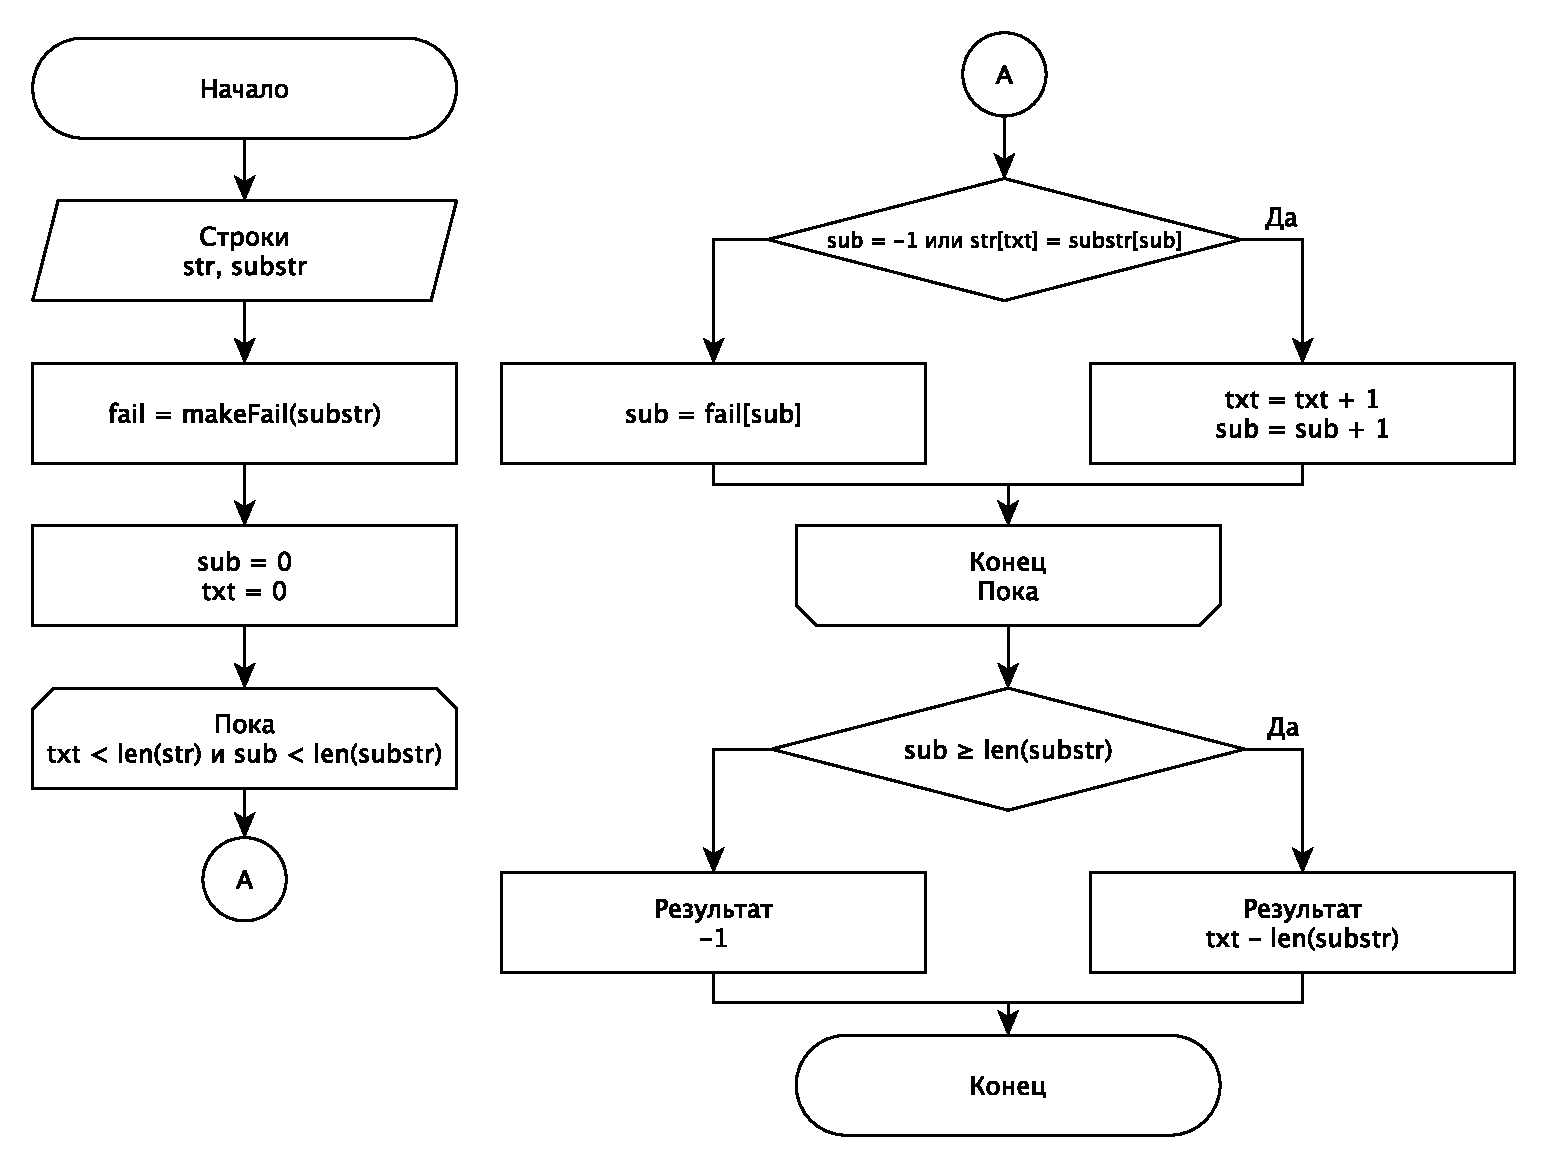
\includegraphics[scale=0.65]{knuth_morris_pratt}
    \caption{Схема алгоритма Кнута-Морриса-Пратта}
    \label{img:kmp}
\end{figure}

\begin{figure}[H]
    \centering
    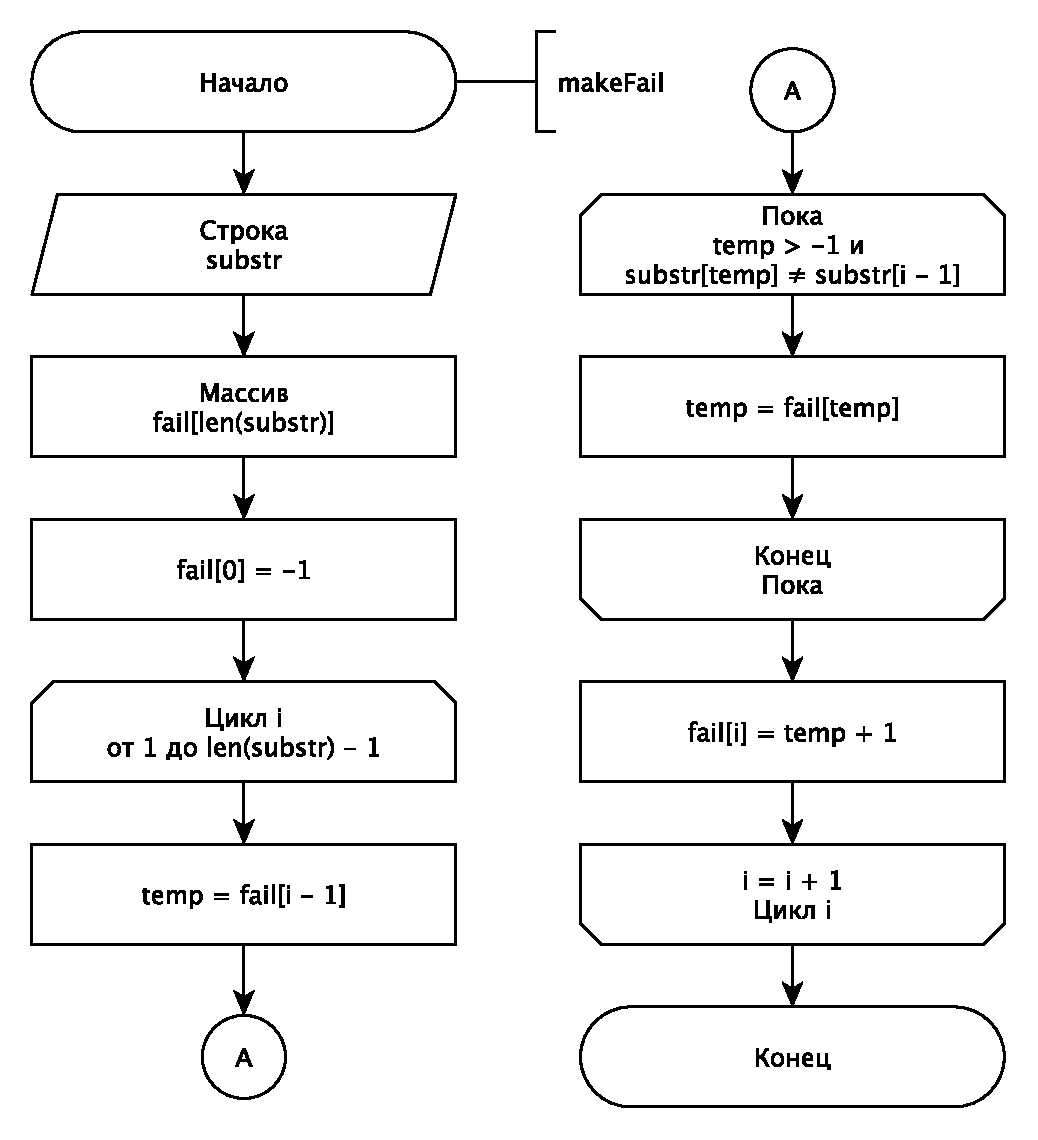
\includegraphics[scale=0.8]{fail}
    \caption{Схема алгоритма создания массива сдвигов}
    \label{img:fail}
\end{figure}

\begin{figure}[H]
    \centering
    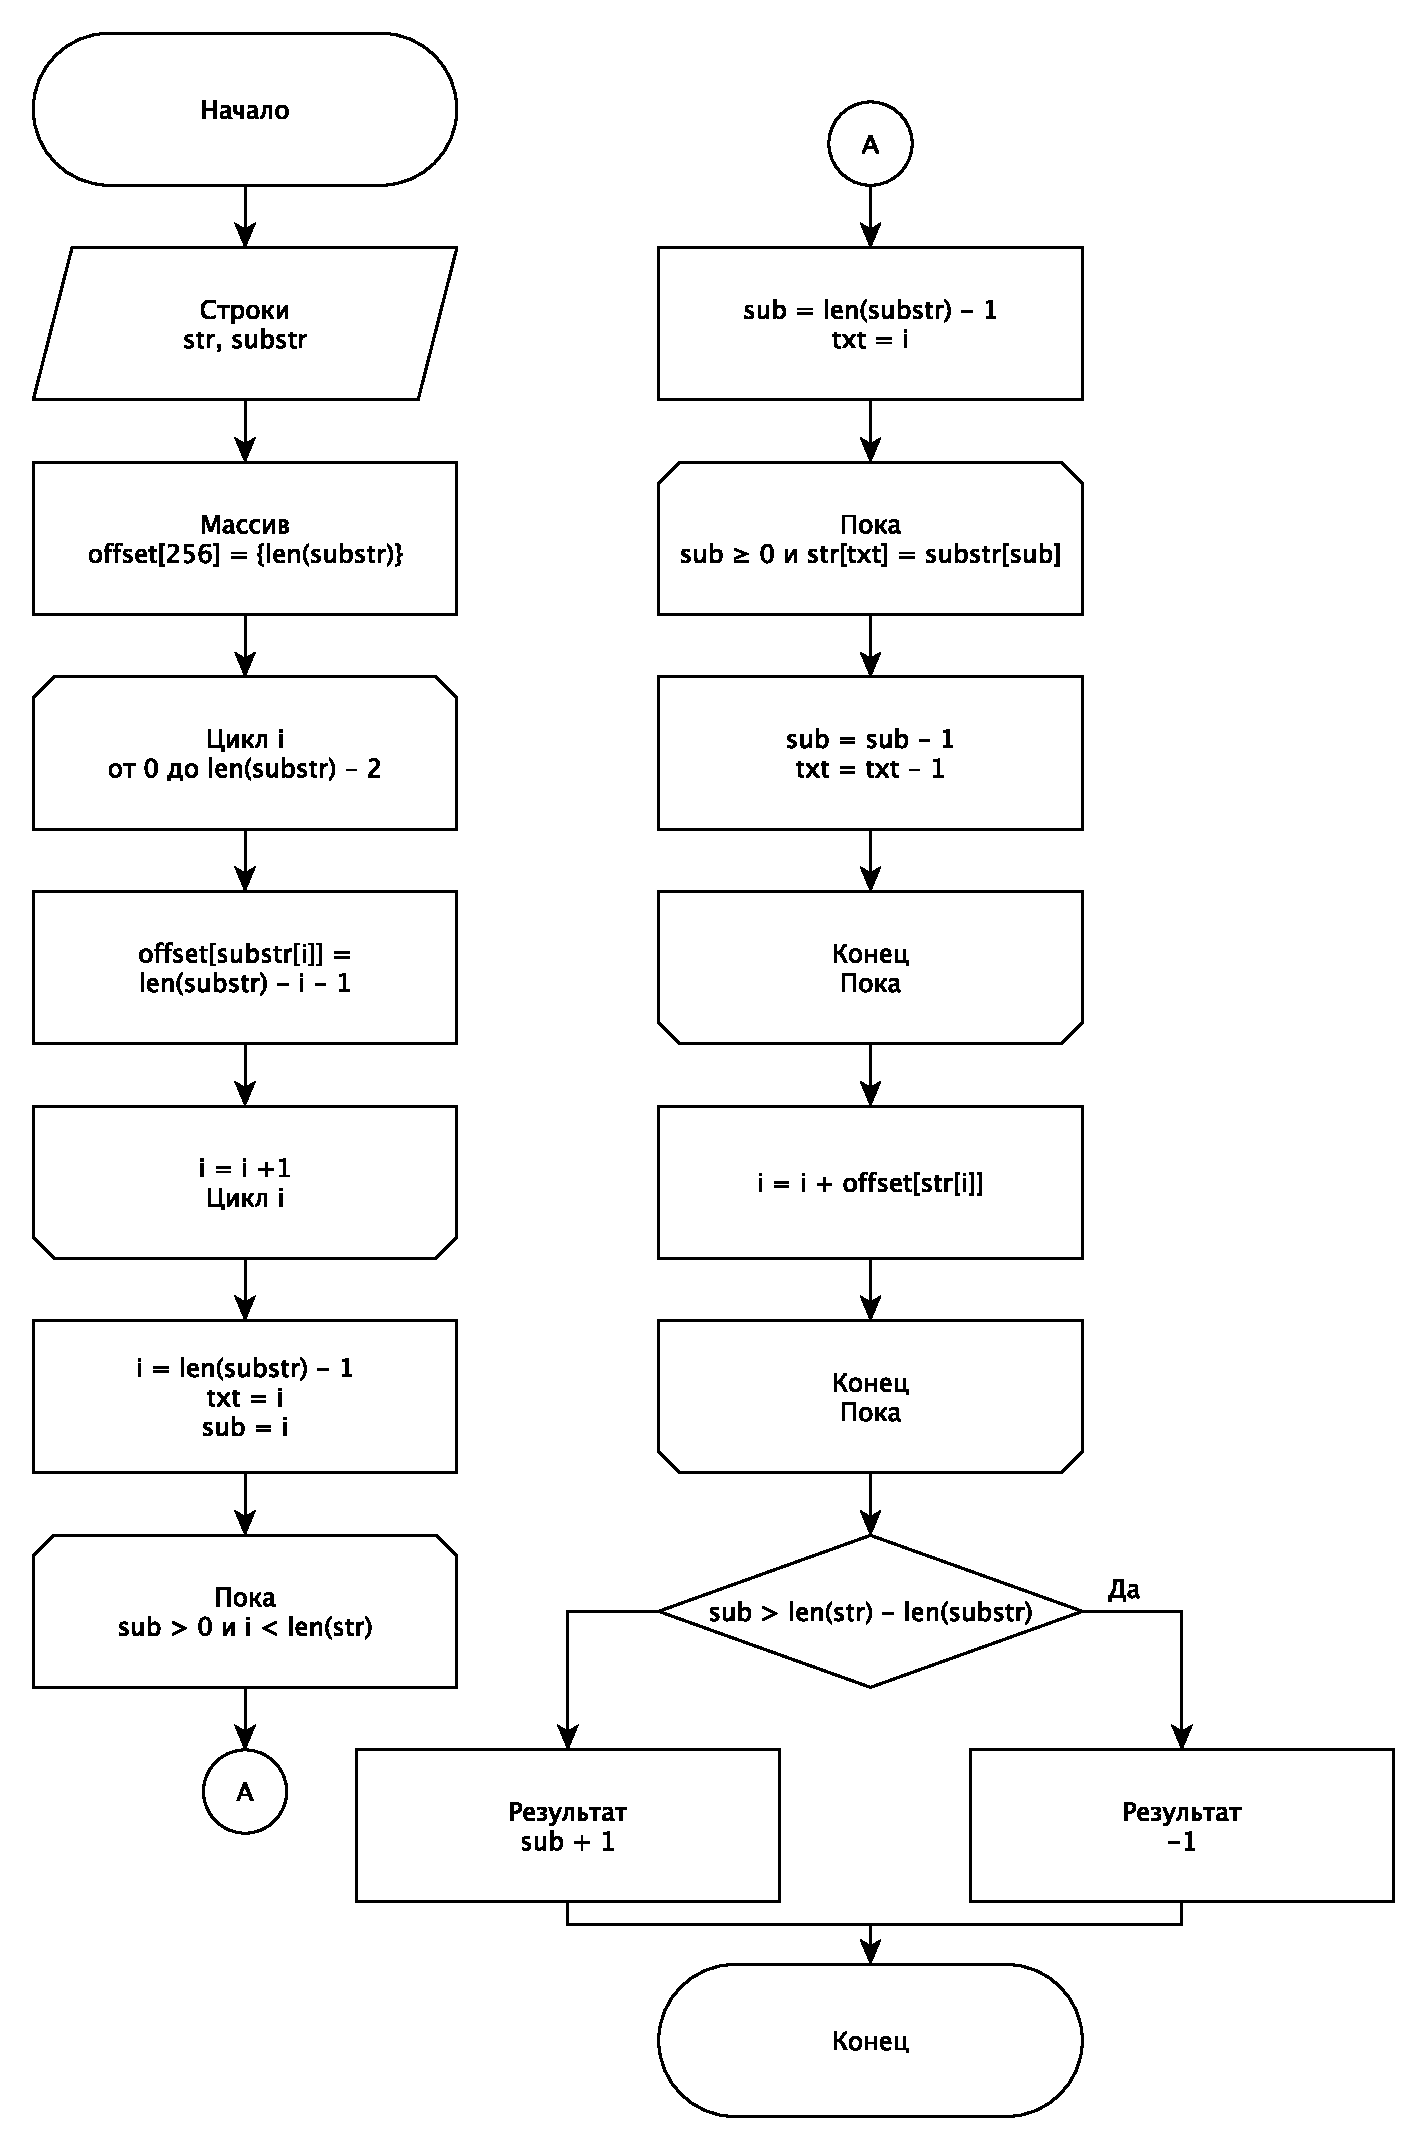
\includegraphics[scale=0.6]{boiler_myr}
    \caption{Схема алгоритма Бойлера-Мура}
    \label{img:bm}
\end{figure}

\subsection{Выводы}

Изучены алгоритмы поиска подстроки в строке, необходимо их реализовать.

\newpage
\section{Технологическая часть}

Стоит задача реализовать алгоритмы поиска подстроки в строке.

\subsection{Средства реализации}

В качестве языка программирования был выбран {\ttfamily C++}.
Данный язык имеет высокую скорость и богатую стандартную библиотеку,
содержащую необходимые контейнеры для данной работы. Программа, написанная на
{\ttfamily C++}, будет доступна на всех платформах.

\subsection{Листинг кода}

На листингах \ref{lst:kmp} и \ref{lst:bm} предсавлены алгоритмы
Кнута-Морриса-Пратта и Бойлера-Мура. На листинге \ref{lst:fail} представлен
алгоритм создания массива сдвигов для алгоритма Кнута-Морриса-Пратта.

\begin{lstlisting}[caption=Алгоритм Кнута-Морриса-Пратта,label=lst:kmp]
int KnuthMorrisPratt::find(const std::string& str,
                           const std::string& substr)
{
    if (substr.size() > str.size()) return -1;

    std::vector< int > fail = makeFail(substr);

    int sub = 0;
    int txt = 0;

    while (txt < int(str.size()) && sub < int(substr.size())) {
        if (sub == -1 || str[txt] == substr[sub]) {
            ++txt;
            ++sub;
        } else {
            sub = fail[sub];
        }
    }

    if (sub >= substr.size())
        return txt - substr.size();

    return -1;
}
\end{lstlisting}

\begin{lstlisting}[caption=Алгоритм создания массива сдвигов,label=lst:fail]
std::vector< int > KnuthMorrisPratt::makeFail(
    const std::string& substr
)
{
    std::vector< int > fail(substr.size());

    fail[0] = -1;

    for (int i = 1; i < fail.size(); ++i) {
        int temp = fail[i - 1];

        while (temp > -1 && substr[temp] != substr[i - 1]) {
            temp = fail[temp];
        }

        fail[i] = temp + 1;
    }

    return fail;
}
\end{lstlisting}

\begin{lstlisting}[caption=Алгоритм Бойлера-Мура,label=lst:bm]
int BoilerMyr::find(const std::string& str, const std::string& substr)
{
    if (substr.size() > str.size()) return -1;

    std::vector< int > offset;

    for (int i = 0; i <= 255; ++i) {
        offset.push_back(int(substr.size()));
    }

    for (int i = 0; i < substr.size() - 1; ++i) {
        offset[int(substr[i])] = substr.size() - i - 1;
    }

    int i = int(substr.size()) - 1;
    int txt = i;
    int sub = i;

    while (txt > 0 && i < int(str.size())) {
        txt = int(substr.size()) - 1;
        sub = i;

        while (txt >= 0 && str[sub] == substr[txt]) {
            --sub;
            --txt;
        }

        i += offset[int(str[i])];
    }

    if (sub > int(str.size()) - int(substr.size())) return -1;

    return sub + 1;
}
\end{lstlisting}

\subsection{Тестирование}

Для тестирования были заготовлены следующие тесты, которые представлены
на таблице \ref{table:test}.

\begin{table}[H]
    \caption{Тесты}
    \label{table:test}
    \centering
    \begin{tabular}{|c|c||c|}
        \hline
        Строка & Подстрока & Ожидаемый результат \\
        \hline
        \hline
        abababbc & ababbc & 2 \\
        \hline
        qwe & qwe & 0 \\
        \hline
        asdasd & sa & -1 \\
        \hline
        abababa & baba & 1 \\
        \hline
    \end{tabular}
\end{table}

\subsection{Выводы}

Были реализованы алгоритмы поиска подстроки в строке и подготовлены тесты.

\newpage
\section{Экспериментальная часть}

Необходимо протестировать написанную программу.

\subsection{Примеры работы}

Примеры работы программы представлены на рисунках
\ref{img:zero_arg}, \ref{img:good}, \ref{img:not_found}.

\begin{figure}[H]
    \centering
    
\includegraphics[scale=0.4]{zero_arg}
    \caption{Пример работы без аргументов}
    \label{img:zero_arg}
\end{figure}

\begin{figure}[H]
    \centering
    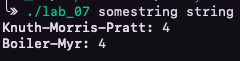
\includegraphics[scale=0.8]{good}
    \caption{Пример работы с найденной подстрокой}
    \label{img:good}
\end{figure}

\begin{figure}[H]
    \centering
    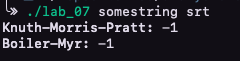
\includegraphics[scale=0.8]{not_found}
    \caption{Пример работы без подстроки}
    \label{img:not_found}
\end{figure}

\subsection{Результаты тестирования}

Результаты тестирования представлены на таблице \ref{table:test_result}.

\begin{table}[H]
    \caption{Результаты}
    \label{table:test_result}
    \centering
    \begin{tabular}{|c|c||c|c|}
        \hline
        Строка & Подстрока & Результат работы КМП & Результат работы БМ \\
        \hline
        \hline
        abababbc & ababbc & 2 & 2\\
        \hline
        qwe & qwe & 0 & 0\\
        \hline
        asdasd & sa & -1 & -1 \\
        \hline
        abababa & baba & 1 & 1 \\
        \hline
    \end{tabular}
\end{table}

Все тесты пройдены успешно.

\subsection{Выводы}

Написанная программа прошла все тесты успешно.

\newpage
\anonsection{Заключение}

В данной работе были изучены и разработаны алгоритмы поиска
подстроки в строке Кнута-Морриса-Пратта и Бойлера-Мура.

Следующие задачи были выполнены:

\begin{itemize}
    \item изучены основные алгоритмы, решающих задачу поиска;
    \item реализованы данные алгоритмы.
\end{itemize}

\newpage
\addcontentsline{toc}{section}{Список используемой литературы}

\begin{thebibliography}{}
    \bibitem{office} Поиск текста в документе [Электронный ресурс] -- Режим доступа: https://support.office.com/ru-ru/article/Поиск-текста-в-документе-672d56af-7ad9-4b98-872c-ceed9c81c21c Дата обращения: 18.12.2019

    \bibitem{cpp} Документация по find [Электронный ресурс] -- Режим доступа: https://ru.cppreference.com/w/cpp/string/basic string/find Дата обращения: 18.12.2019
\end{thebibliography}

\end{document}
